\documentclass[10pt,final,journal,a4paper,oneside,twocolumn]{IEEEtran}
\usepackage{graphicx}
\usepackage{multirow}
\usepackage{xcolor, soul}  
\usepackage{indentfirst}
\usepackage{float}
\usepackage{caption}

\renewcommand\IEEEkeywordsname{Keywords}

\title{Decentralized and Secure Voting System using Blockchain Technology}
\author{
  Arvind Sudarshan,
  Chatane Shree Atul,
  Eksambekar Yash Sagar,
  Gadkari Gaurav Sudhir
}

\begin{document}

	\maketitle

	\begin{abstract}
		Voting in democratic country is a fundamental right granted to every eligible individual by the constitution. Current e-Voting system used isn’t transparent and can be improved in a few aspects. All voting data from Electronic Voting Machines (EVMs) are stored on a central server. This creates a single point of failure which can be exploited and tampered with easily. Such flaws cause mistrust in the electoral process. Blockchain is a shared immutable ledger that facilitates the process of recording transactions in a network. It is an emerging technology whose full potential is yet to be realized. Blockchain became popular in 2009 when bitcoin was introduced and used as an alternative to tangible currency and has evolved since. It is a reliable system that can be used in various critical industrial applications. Blockchain has potential to improve the voting system to contest transparent and fair voting. Using this modern technology, a voting system can be implemented which provides transparency leading to fairness in the system. Furthermore, this will overcome the current system flaw of having a single point of failure caused by storing data in a centralized server. In addition to this, election results can be declared faster compared to the current system which might take a few days. The proposed system in this paper shows implementation of voting using blockchain technology.
	\end{abstract}

	\begin{IEEEkeywords}
		Blockchain Technology, Ethereum Virtual Machine, Voting System, Secure Voting, Consensus
	\end{IEEEkeywords}
	
	\section{Introduction}
		To conduct a fair election and lessen unfairness, blockchain technology can be integrated into the electronic voting system. Similar to how computerized voting systems aren't perfect enough to be used on a broad scale, physical voting systems have several problems. An overview of blockchain-based voting systems is provided in this paper. By using blockchain, the proposed platform will offer a framework that can be used to carry out voting operations electronically. We're going to use a customizable blockchain with consensus methods for our system. Voting transactions are more integrated and secure thanks to the chain security algorithm.
		\\\textbf{Blockchain:} Blockchain is a distributed ledger technology that links together blocks, or records of transactions, using mathematical cryptography. The distributed aspect of blockchain technology, which renders it immutable and virtually hard to hack, is what makes it so popular.
		\\\textbf{Distributed Ledger:} A ledger is a collection of records that details transactions. A distributed ledger is a data structure that may be used to store transactions and is spread over numerous computers connected to a network. Distributed ledger technology, or DLT, is a method of distributing transaction records to any user connected to the network. A sort of distributed ledger technology is blockchain. As a result, all of its users have access to the data, which promotes transparency and eliminates corruption.
		\\\textbf{Decentralized Application(dApp):} A decentralized application (dApp) is a programme designed to function on a distributed ledger technology, such as a blockchain. Smart contracts are used by it to operate.
		\\\textbf{Smart Contract:} Computer programmes known as "smart contracts" automatically carry out or regulate actions in accordance with the terms of a contract or other agreement. It is applied to blockchain transactions to impose rules. The essential building blocks of cryptocurrencies and NFTs are thought to be smart contracts.
		\\\textbf{Consensus:} Consensus makes sure that all the various blockchain participants reach a consensus regarding the state of the blockchain. Different blockchain applications employ a variety of consensus mechanisms.
		\\\textbf{Cryptography:} Computer science and mathematical theory are the foundations of cryptography. The purpose of cryptography is to provide means of applying techniques linked to encryption to secure and safeguard data and communications.
		\\\textbf{Ethereum:} The open-source Ethereum blockchain uses the solidity programming language to support smart contracts.

	\section{Background and Related Work}

		\subsection{A Framework to Make Voting System Transparent Using Blockchain Technology \cite{farooq2022framework}}
			\begin{enumerate}
				\item The transparent voting mechanism using blockchain technology is explained in this paper. It drastically cuts down on the resources and labor used in the voting process. Voting systems built on the blockchain are resistant to manipulation, unlike traditional voting systems that save votes on a centralized database. Compared to earlier technologies, blockchain offers a high level of security that can be trusted more.
				\item Here, voters must finish the voting management system's verification process. To maintain the integrity of voters, the system's database is integrated with the country's database. A transaction is created for each vote and checked against the voter's National ID before being recorded in the blockchain. The voter uses their vote currency after casting a ballot. Blockchain checks his voting system after casting a ballot against the national voting IDs. Then, before adding them to the chain, miners examine them to weed out malicious votes.
			\end{enumerate}

		\subsection{An Empirical Analysis Of Using Blockchain Technology In E-Voting Systems \cite{cadiz2021empirical}}
			This study compares and contrasts the performance and security of centralized versus blockchain-based electronic voting systems. Similar interfaces were planned for both systems. The backend design systems were the only thing separating them. With blockchain-based systems, users have to join the network using the private key of their digital wallet as their credentials. A new block is created, processed, and then added to the blockchain, which acts as the system's database, if all the terms of the contract are met. Users had to sign in to the centralized system using their voter ID. The votes are tallied automatically for each candidate after being processed by the server and saved in a database. The findings indicated that BEVS is somewhat slower than CEVS. This is because a local private blockchain handles queries more quickly than a public blockchain network due to the additional block production and validation operations. However, the BEVS is more efficient and reliable than the CEVS because it runs through the internal server and has a zero error rate. Even with heavy loads, the BEVS's rate of operation can be impacted. With fewer weaknesses found, the BEVS is also proving to be a more secure electronic voting system.

		\subsection{Decentralized E-voting system based on Smart Contract by using Blockchain Technology \cite{al2020decentralized}}
			\begin{enumerate}
				\item This Paper Explains the Difference between Ballot paper voting and Blockchain based decentralized casting For better integrity of the voting system.
				\item Data like a voter's name or their votes are saved on a decentralized ledger in the decentralized blockchain system. No outside authority has access to or has the ability to alter this data. The usage of currency ballot papers as a voting method is commonplace globally. Due to the availability of the data at a single resource, this does not, however, guarantee the accuracy of the outcome. Blockchain-based voting systems solve the issue that a centralized voting system has. Here, using blockchain technology, data is distributed across various servers and locations rather than being kept in a single location. Using a peer-to-peer network, the data is distributed among all of the hardware connected to the blockchain.
				\item Before voting begins in the Decentralised E-voting system, candidates must register, and voters' identities must first be confirmed before accounts may be created.within this system. Following voter authentication by an authorized party, blockchain makes sure that voting twice is not permitted.
			\end{enumerate}

		\subsection{An Architecture of Blockchain based Voting System \cite{angsuchotmetee2019blockvote}}
			The study suggests BlockVOTE, a Blockchain-based voting system. It focuses on employing consensus handling procedures to maintain the voting system's security and dependability. The drawbacks with both traditional ballot-based voting methods and electronic voting systems are discussed in the article. The study defines upon processes Poll Creation, Voting, and Result Tallying in the suggested architecture. The system was constructed by the paper's authors using Ethereum and HyperLedger, and the outcomes were compared. The system will contain the following actors executing duties related to poll creation, contract development and deployment, and voting: poll creator, contract handler, and voter.
			\begin{figure}[H]
				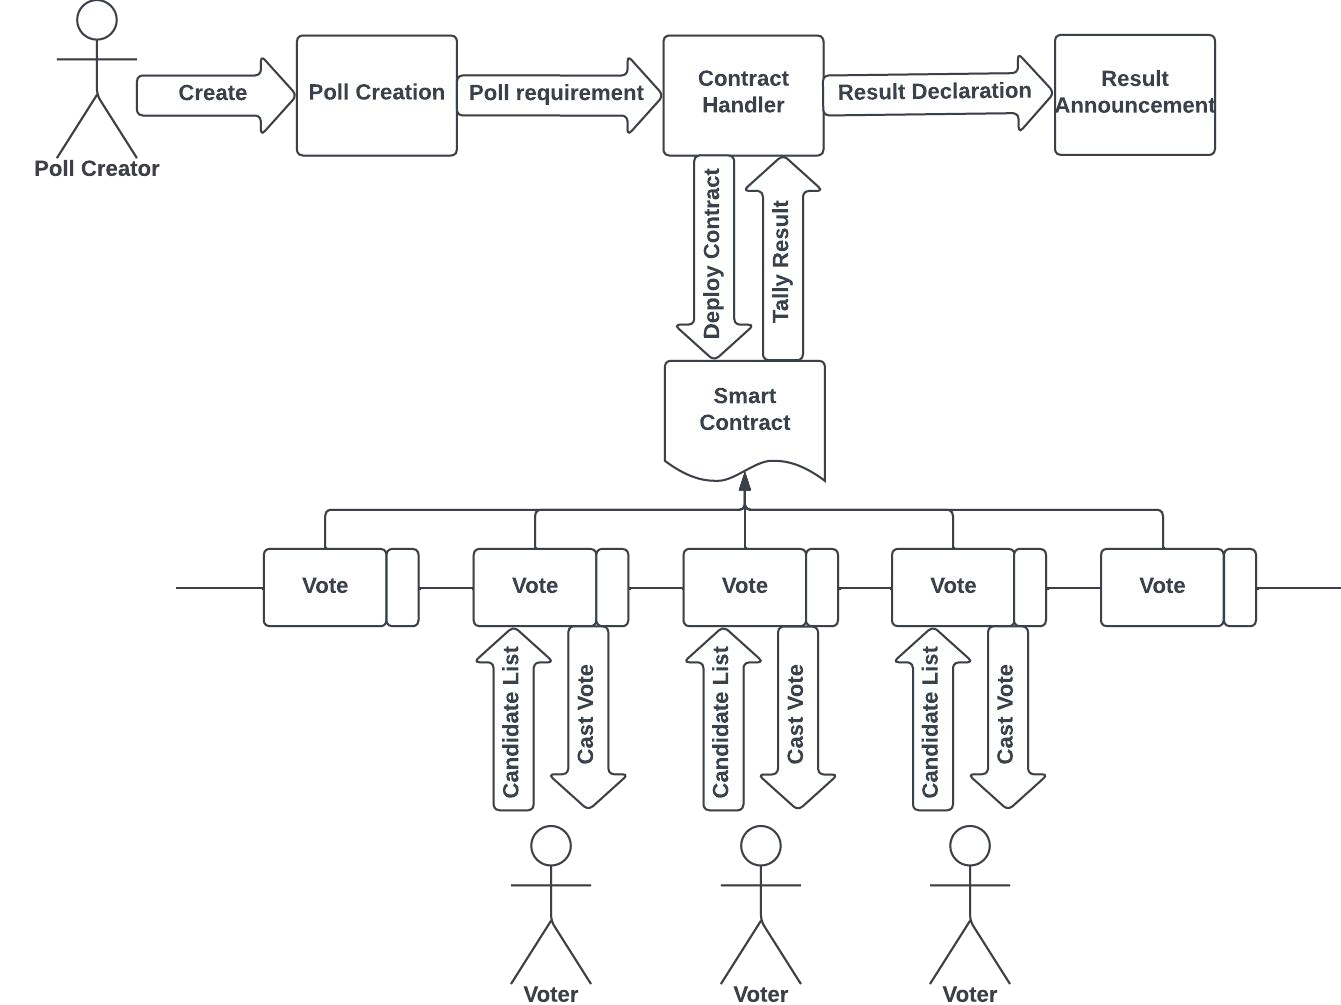
\includegraphics[width=\linewidth]{./Resources/architecture.png}
			    \caption{Blockchain based e-Voting Architecture}
			\end{figure}

		\subsection{Analysis of Blockchain Solutions for E-Voting: A Systematic Literature Review \cite{benabdallah2022analysis}}
			This study examines the most recent advancements in the blockchain-based electronic voting system to comprehend their specifics and contrasts them with each other and the conventional voting process. Here, various blockchain-based e-voting apps are evaluated based on a variety of factors, including the implementations utilized, the algorithms employed, the methods used to identify voters and encrypt votes, their resilience to assaults, and other security-related factors. After comparing these based on the aforementioned characteristics, these systems' shortcomings and restrictions. Even though the blockchain-based voting systems are still in their infancy, they present an intriguing alternative to the drawbacks of conventional voting.

		\subsection{Blockchain Based E-Voting System: Open Issues and Challenges \cite{khudoykulov2021blockchain}\cite{jafar2021blockchain}}
			\begin{enumerate}
				\item This study examines and critiques recent research on blockchain-based electronic voting systems. E-voting is the process that uses electronic technologies during an election to facilitate voting and vote counting. Every country has a different electronic voting process. which might include electronic voting machines in polling places, central recording of paper votes, and online voting. Centralized calculations are employed in numerous nations. However, in some voting locations, there are also electronic voting machines and internet voting is hardly ever used. Particularly, issues with security and dependability were found when several electronic approaches were tested. Several other aspects of an electronic voting system's security are discussed in this paper, including
					\begin{enumerate}
						\item Anonymity: Any association between the registered voters and their identity must remain anonymous.
						\item Auditability and Accuracy: The outcomes ought to accurately reflect the preferences of the voters.
						\item Democracy/Singularity: Every eligible person should be able to cast a ballot in a democracy/singularity. No votes may be cast more than once.
						\item Vote Privacy:  No one should be able to connect a specific vote to a specific person.
						\item Robustness and Integrity:  This is evidence that legitimate registered voters will easily abstain from voting. Additionally, it inspires others to exercise their right to vote.
						\item Transparency and Fairness:  The results are kept secret from those not directly involved in the counting process until they are released.
						\item Availability and Mobility: The systems must be accessible at all times during the election.
						\item Verifiable Participation/Authenticity: If a voter chooses not to cast a ballot, it should be possible for the authorities to determine this.
						\item Recoverability and Identification: To prevent attacks or data losses, it should be able to track down and retrieve data.
					\end{enumerate}
					\begin{figure}[H]
						\centering
						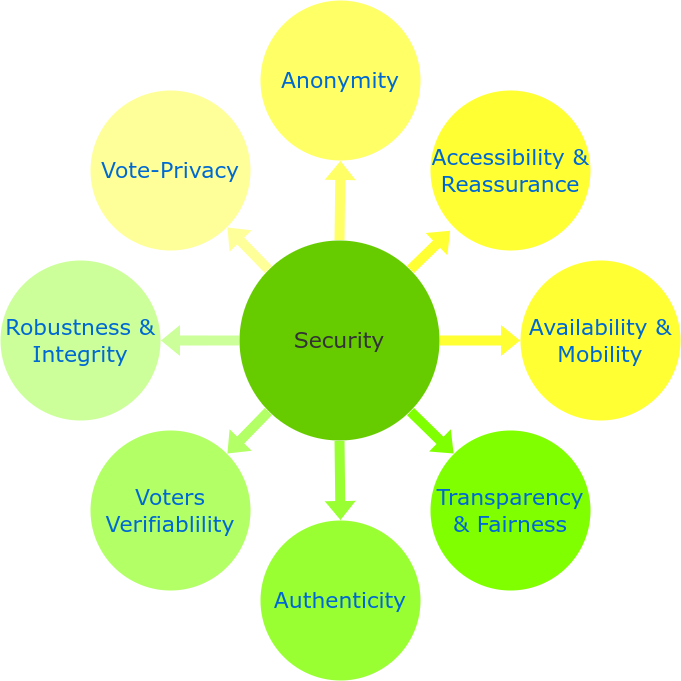
\includegraphics[width=\linewidth]{./Resources/security-requirements.png}
					    \caption{Security Requirements for Electronic Voting System}
					\end{figure}
				\item  The following elements are found in a blockchain:
					\begin{enumerate}
						\item Node: It describes a user or computer connected to the blockchain network.
						\item Transaction: Transactions are the most essential component of a blockchain system since they are the data that is kept in blocks.
						\item Block: The data structure known as a block is used to store transactional information.
						\item Chain: A series of transaction blocks arranged in a particular order.
						\item Miners: Particular nodes that carry out block verification.
						\item Consensus: An algorithm that determines whether a block should be added into the chain and ensures its validity.
					\end{enumerate}
					\begin{figure}[H]
						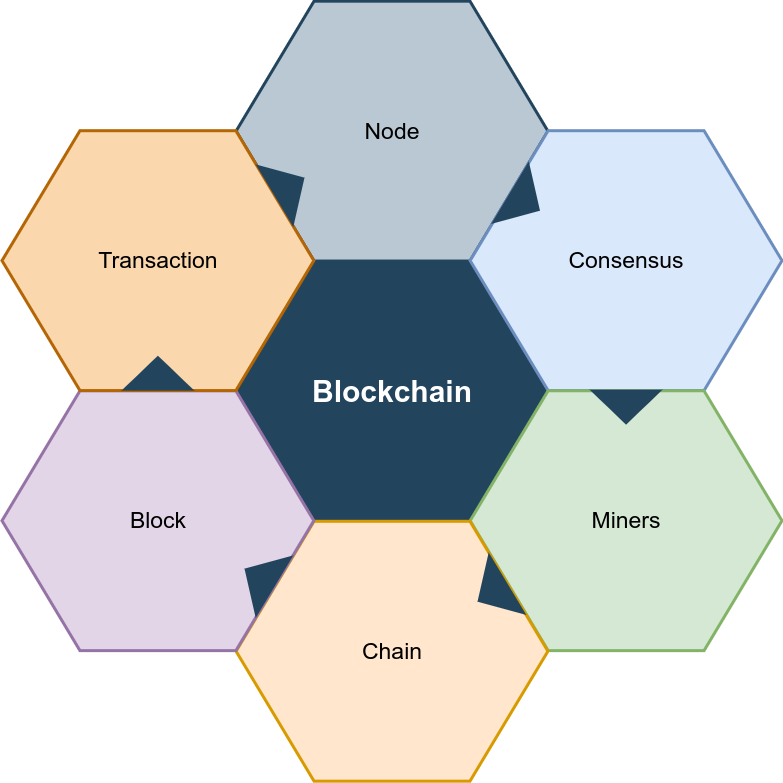
\includegraphics[width=\linewidth]{./Resources/core-components.png}
					    \caption{Core Components of Blockchain Architecture}
					\end{figure}
			\end{enumerate}

	\section{Methodology}
		To implement and test a blockchain based voting system, a few components have to be designed. A privately hosted closed blockchain network is required for our contract to run on. This is created using ethereum’s Go language based client. To do so, a script is written in JavaScript to automate the following tasks :
		\\\\\colorbox{gray!20}{%
	        \begin{minipage}{\linewidth}%
	            \vspace*{2pt}
	           	\begin{enumerate}
	           		\item Ethereum wallet accounts are created for the number of nodes required.
	           		\item On these accounts, the genesis block is initialized.
	           		\item Bootnode is initialized. Bootnode is a node which connects other nodes to each other.
	           		\item Geth (Go Ethereum Client) is run using the accounts created using bootnode initialized in the previous step.
	           	\end{enumerate}
	            \vspace*{2pt}
	        \end{minipage}%
	    }
		\\\\\\A Solidity based contract is written to execute the application’s core functionality. This contract works like the backend for the entire application. This contract is written in solidity version 0.8.19 :
		\\\\\colorbox{gray!20}{%
	        \begin{minipage}{\linewidth}%
	            \vspace*{2pt}
				ElectoralContract \{
					\\\\\-\hspace{1cm}struct Voter \{
						\\\-\hspace{2cm}string voterName;
						\\\-\hspace{2cm}bool hasVoted;
						\\\-\hspace{2cm}bool isLoggedIn;
						\\\-\hspace{2cm}string voterPassword;
						\\\-\hspace{2cm}address nodeAddress;
						\\\-\hspace{2cm}uint timestamp;
					\\\-\hspace{1cm}\}
					\\\\\-\hspace{1cm}struct Candidate \{
						\\\-\hspace{2cm}string candidateName;
						\\\-\hspace{2cm}uint256 voteCount;
					\\\-\hspace{1cm}\}
					\\\\\-\hspace{1cm}// func addCandidate : adds candidate for voters to vote
					\\\-\hspace{1cm}// func addVoter : adds voter
					\\\-\hspace{1cm}// func login : login functionality for voter
					\\\-\hspace{1cm}// func logout : logout functionality for voter
					\\\-\hspace{1cm}// func getResult : gets result of elections
					\\\-\hspace{1cm}// func getCandidates : gets list of candidate names
					\\\-\hspace{1cm}// func getVotersDetailed : gets all voters information
					\\\-\hspace{1cm}// func vote : cast vote to candidate functionality
				\\\\\};
	            \vspace*{2pt}
	        \end{minipage}%
	    }
		\\\\\\Algorithm to cast vote :
		\\\\\colorbox{gray!20}{%
	        \begin{minipage}{\linewidth}%
	            \vspace*{2pt}
				\begin{table}[H]
					\resizebox{\textwidth}{!}{%
						\begin{tabular}{llll}
							Require & : & Voter must have not cast vote earlier &                                     \\
							Require & : & Voter must be logged in               &                                     \\
							Update  & : & candidate.voteCount++                 & //Update vote count for candidate   \\
							Update  & : & voter.hasVoted = true                 & //Update voting status for voter    \\
							Update  & : & voter.timestamp = timestamp           & //Update voting timestamp for voter \\
							Func    & : & logout(voterId)                       & //Logout voter                     
						\end{tabular}%
					}
				\end{table}
	            \vspace*{2pt}
	        \end{minipage}%
	    }
		\\\\\\The overall flow followed is :
		\begin{figure}[H]
			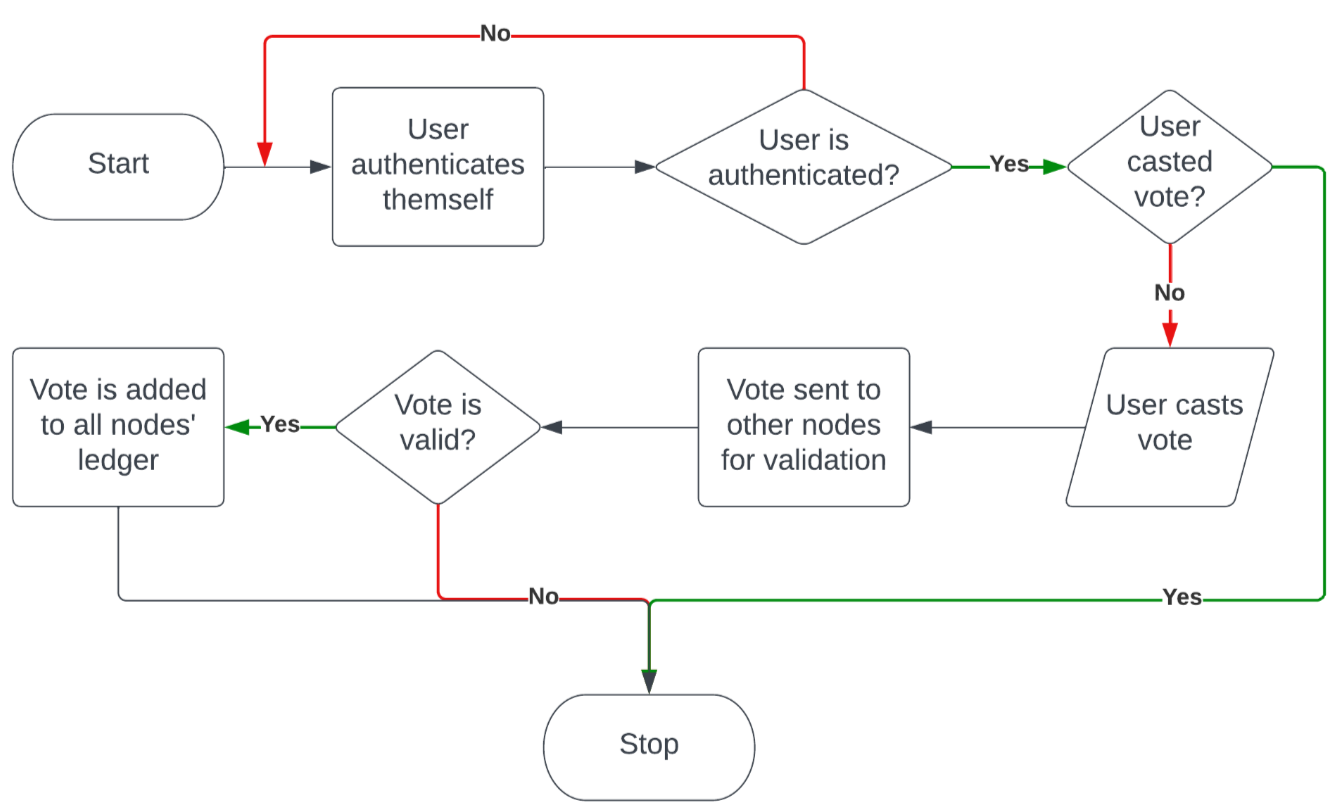
\includegraphics[width=\linewidth]{./Resources/flow.png}
		    \caption{Flow of the system}
		\end{figure}
		Consensus algorithm used in this chain is Proof of Authority (Clique). In PoA consensus, some nodes are given permission to generate new blocks. These nodes are called ‘Validators’. PoA leverages the importance of identities. The validators are not staking coins like PoS but rather their own reputation instead. PoA is suited for private networks such as this one.
		\\\\Finally, to evaluate the system, some synthetic data is generated and provided to the system and performances tested. To perform this evaluation, python script is written which will perform these tasks :
		\\\\\colorbox{gray!20}{%
	        \begin{minipage}{\linewidth}%
	            \vspace*{2pt}
            	\begin{enumerate}
            		\item Register a single candidate.
            		\item Register required number of voters with random names.
            		\item Login with all voters’ credentials.
	           		\item Cast votes by voters with preset probability.
	           		\item Logout all logged in voters.
	           		\item Get result and compile csv.
            		\item Plot graphs from results.
            	\end{enumerate}
	            \vspace*{2pt}
	        \end{minipage}%
    	}
	    \\\\\\Along with these components, a frontend client is made for a citizen/voter to interact and cast their votes. Dashboards are also deployed to monitor the network and the data flowing through it. The system’s performance is tested by generating synthetic data which is passed to the system and the time taken for it to process the data and store it in blockchain. The number of nodes in the system are scaled in range from 1 to 50 while ranging the voters from 10 to 250.

	\section{Results}
		Table \ref{tab:result-table} shows time taken in seconds by the system to insert data to the private blockchain network and generate results without artificial delay included.
		\begin{table*}
			\centering
			\caption{Time Taken - (Number Of Nodes Vs Voters)}
			\label{tab:result-table}
			\begin{tabular}{|cr|rrrrrrrrrr|}
				\hline
				\multicolumn{2}{|c|}{\multirow{2}{*}{}}       & \multicolumn{10}{c|}{Number of nodes}                                                                                                                                                                                                                                              \\ \cline{3-12} 
				\multicolumn{2}{|c|}{}                        & \multicolumn{1}{r|}{1}     & \multicolumn{1}{r|}{2}      & \multicolumn{1}{r|}{3}     & \multicolumn{1}{r|}{4}      & \multicolumn{1}{r|}{5}      & \multicolumn{1}{r|}{10}     & \multicolumn{1}{r|}{15}     & \multicolumn{1}{r|}{20}     & \multicolumn{1}{r|}{25}     & 50     \\ \hline
				\multicolumn{1}{|c|}{\multirow{4}{*}{}} & 10  & \multicolumn{1}{r|}{0.46}  & \multicolumn{1}{r|}{7.08}   & \multicolumn{1}{r|}{2.4}   & \multicolumn{1}{r|}{5.89}   & \multicolumn{1}{r|}{20.26}  & \multicolumn{1}{r|}{6.27}   & \multicolumn{1}{r|}{6.76}   & \multicolumn{1}{r|}{10.15}  & \multicolumn{1}{r|}{5.94}   & 4.84   \\ \cline{2-12} 
				\multicolumn{1}{|c|}{}                  & 20  & \multicolumn{1}{r|}{0.9}   & \multicolumn{1}{r|}{13.56}  & \multicolumn{1}{r|}{3.75}  & \multicolumn{1}{r|}{5.97}   & \multicolumn{1}{r|}{35.4}   & \multicolumn{1}{r|}{13.16}  & \multicolumn{1}{r|}{17.4}   & \multicolumn{1}{r|}{14.87}  & \multicolumn{1}{r|}{12.44}  & 56.11  \\ \cline{2-12} 
				\multicolumn{1}{|c|}{}                  & 30  & \multicolumn{1}{r|}{1.33}  & \multicolumn{1}{r|}{19.15}  & \multicolumn{1}{r|}{6.16}  & \multicolumn{1}{r|}{10.16}  & \multicolumn{1}{r|}{45.24}  & \multicolumn{1}{r|}{81.77}  & \multicolumn{1}{r|}{22.4}   & \multicolumn{1}{r|}{19.29}  & \multicolumn{1}{r|}{19.11}  & 41.7   \\ \cline{2-12} 
				\multicolumn{1}{|c|}{}                  & 40  & \multicolumn{1}{r|}{1.76}  & \multicolumn{1}{r|}{8.88}   & \multicolumn{1}{r|}{9.25}  & \multicolumn{1}{r|}{13.58}  & \multicolumn{1}{r|}{61}     & \multicolumn{1}{r|}{31.21}  & \multicolumn{1}{r|}{30.11}  & \multicolumn{1}{r|}{31.57}  & \multicolumn{1}{r|}{29.68}  & 33.01  \\ \cline{2-12} 
				\multicolumn{1}{|c|}{Voters}            & 50  & \multicolumn{1}{r|}{2.3}   & \multicolumn{1}{r|}{35.77}  & \multicolumn{1}{r|}{11.73} & \multicolumn{1}{r|}{15}     & \multicolumn{1}{r|}{65.16}  & \multicolumn{1}{r|}{43.83}  & \multicolumn{1}{r|}{39.35}  & \multicolumn{1}{r|}{37.42}  & \multicolumn{1}{r|}{32.23}  & 28.8   \\ \cline{2-12} 
				\multicolumn{1}{|c|}{\multirow{4}{*}{}} & 100 & \multicolumn{1}{r|}{4.61}  & \multicolumn{1}{r|}{22.82}  & \multicolumn{1}{r|}{21.81} & \multicolumn{1}{r|}{30.53}  & \multicolumn{1}{r|}{139.74} & \multicolumn{1}{r|}{87.84}  & \multicolumn{1}{r|}{71.14}  & \multicolumn{1}{r|}{77.71}  & \multicolumn{1}{r|}{70.99}  & 111.91 \\ \cline{2-12} 
				\multicolumn{1}{|c|}{}                  & 150 & \multicolumn{1}{r|}{7.93}  & \multicolumn{1}{r|}{35.41}  & \multicolumn{1}{r|}{34.93} & \multicolumn{1}{r|}{45.02}  & \multicolumn{1}{r|}{166.75} & \multicolumn{1}{r|}{100.94} & \multicolumn{1}{r|}{113.08} & \multicolumn{1}{r|}{112.71} & \multicolumn{1}{r|}{111.59} & 161.79 \\ \cline{2-12} 
				\multicolumn{1}{|c|}{}                  & 200 & \multicolumn{1}{r|}{11.18} & \multicolumn{1}{r|}{49.99}  & \multicolumn{1}{r|}{46.33} & \multicolumn{1}{r|}{72.57}  & \multicolumn{1}{r|}{-}      & \multicolumn{1}{r|}{167.5}  & \multicolumn{1}{r|}{143.24} & \multicolumn{1}{r|}{164.77} & \multicolumn{1}{r|}{155}    & 273.67 \\ \cline{2-12} 
				\multicolumn{1}{|c|}{}                  & 250 & \multicolumn{1}{r|}{13.34} & \multicolumn{1}{r|}{152.75} & \multicolumn{1}{r|}{59.7}  & \multicolumn{1}{r|}{105.66} & \multicolumn{1}{r|}{-}      & \multicolumn{1}{r|}{191.49} & \multicolumn{1}{r|}{169.56} & \multicolumn{1}{r|}{189.36} & \multicolumn{1}{r|}{184.24} & 209.19 \\ \hline
			\end{tabular}
		\end{table*}
		
		During evaluation of the system, we faced many failures due to block creation taking a long time, blockchain not being synchronized properly across the network, running out of resources for mining and some unexpected system crashes. Due to these crashes, results for 5 nodes, 200 and 250 voters could not be obtained.

	\section{Conclusion}
		Through the numerous trial runs and performance testing, we were able to make a few observations. These observations were made based on the performance table in the Result section and self experiences while evaluating the system.
		\begin{enumerate}
			\item As the number of voters increases a gradual increase is observed in time taken to insert transactions and get results.
			\item The time taken also increases as the number of nodes in the system is increased. This is due to blockchain synchronization across the network.
			\item Less number of nodes showed instability and frequent crashes since load not being distributed well enough. As the nodes increased, the stability increased and less crashes were observed.
		\end{enumerate}
		From the observations, we can say that voting using blockchain technology is feasible and will be beneficial due to its security and distributed nature. Since voting is carried on large scales, it will be stable and solve few issues faced by the current voting system.


	\bibliographystyle{ieeetr}
	\bibliography{References}

\end{document}